% Preamble. Don't worry about it.
\documentclass{article}
\usepackage{setspace,graphicx}
\usepackage[utf8]{inputenc}
\usepackage[left=1in,top=1in,right=1in,bottom=1in]{geometry} % Document margins
\onehalfspacing

% Setting the depth for Table of Contents
\setcounter{tocdepth}{1}

\begin{document}

% --- TITLE PAGE ---
\title{Donnervögel Consulting \\ Streamlined Grading System}
\author{\textbf{Phase Lead: Ian Pun} \\ Markus Balaski \\ Stephen Laboucane \\
  Graeme Smith \\ Jordan Toering \\  Colin Woodbury \\ Chazz Young}
\date{\today}
\maketitle
\clearpage
% ------------------

% --- REVISION HISTORY ---
\textbf{Revision History}
\begin{center}
  \begin{tabular}{| c | c | c | l |}
    \hline
    Version & Date & Members & Changes\\
    \hline
    1.0 & 2014 Mar 07 (Fri) & Markus B. & Document created\\
    & & Graeme S. & \\
    & & Jordan T. & \\
    & & Stephen L. & \\
    & & Ian P. & \\
    & & Colin W. & \\
    & & Chazz Y. & \\
    \hline
  \end{tabular}
\end{center}
\clearpage
% ------------------------

% --- TABLE OF CONTENTS ---
\tableofcontents
\clearpage
% -------------------------

% ---
\section{Product Overview}  % 5 Marks
% THIS SHOULD BE 1/2 TO 1 PAGE IN LENGTH!
% Markus will do this.

% ---
\section{Getting Started}
\emph{No contents here.}

\subsection{Software Requirements}

\subsection{Hardware Requirements}

\subsection{Installation}

\subsection{Running the Application}

\subsection{UAT??}

% ---
\section{Functions and User Interface Description}  % 30 Marks total
% This is a very big section.
% 1. How is a function selected?
% 2. How is input entered? (Include pictures)
% 3. What keys need to be pressed?
% 4. What will the user see when a step is performed correctly?
% 5. What will the user see when a step is performed incorrectly? (errors)
\subsection{Login}

\subsection{Landing Page}
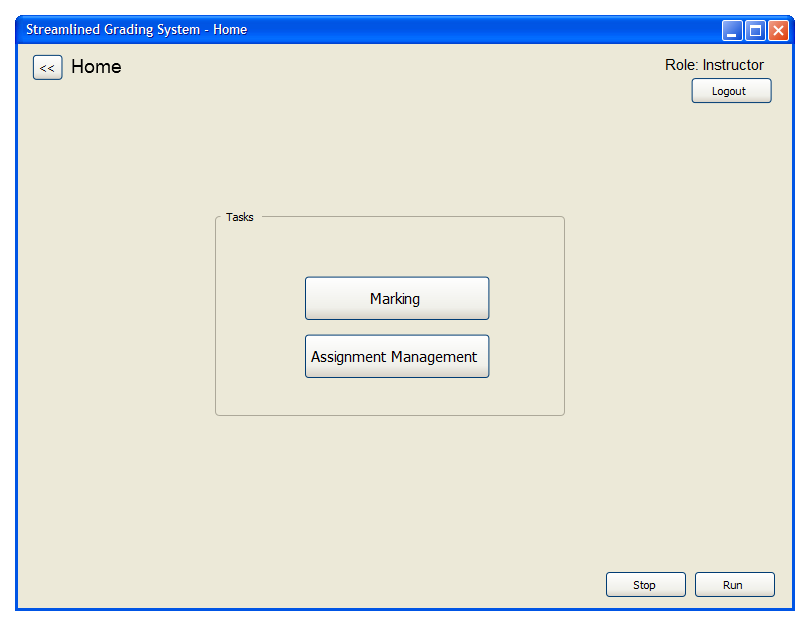
\includegraphics[scale=0.6]{../images/UIMockups/PNG_Renders/LandingPage}
The Landing Page is shown to all users of the system following login.  The Tasks box shows actions that each user can do.  It does not show actions the user cannot do.

\subsection{Manage Courses}

\subsection{Modify Courses}

\subsection{Create/Modify Activity(Detailed)}

\subsection{Copy Activity}

\subsection{Modify Rubric}

\subsection{Activity Marking(Detailed)}
\begin{enumerate}
  \item Log in to the system as a user who has marking privileges.
  \item The following screen will be shown.  Press the \textbf{Marking} button.
  \begin{center} 
   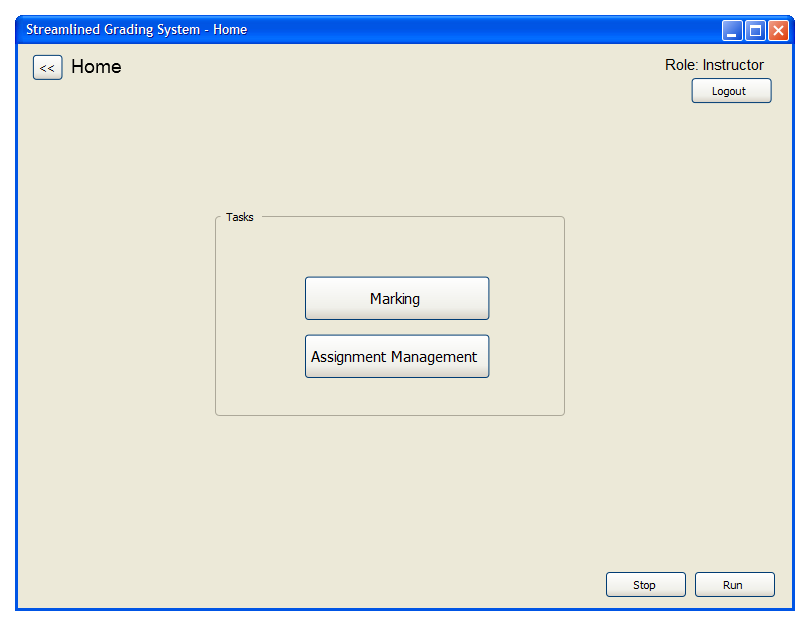
\includegraphics[scale=0.6]{../images/UIMockups/PNG_Renders/LandingPage}
  \end{center}
  \item The following screen will be shown.  Select the course that you wish to do marking for from the drop-down list, then press Ok.
    \begin{center} 
   STEPHEN'S COURSE SELECTION IMAGE HERE
    \end{center}
  \item The following screen will be shown.  Students are listed down the left side.  Available activities are listed along the top.  Find the student you wish to mark for, and select the corresponding activity, then press Ok.
  \begin{center} 
   STEPHEN'S STUDENT/ACTIVITY MATRIX IMAGE HERE
    \end{center}
  \item The assignment's marking screen will be shown.  The marking screen displays the rubric, sample solution, and the student's submission. 
  \begin{center} 
   COLIN'S ASSIGNMENT PAGE HERE
    \end{center}
    Perform the grading process as follows:
    \begin{enumerate}
      \item Perform necessary analysis on the student's work. 
      \item Read rubric points and enter a number into the available box 
      based on your analysis of the student's work.
      \item Repeat step (a) for remaining rubric points.
      \item A total will be shown at the bottom of the rubric to reflect the
       student's final grade on the activity.
      \item Click the \textbf{Submit} button to update the marks database with
      the changes made.
    \end{enumerate}

	\item If desired: Press the \textbf{Submit} button to move to the next student's
	submission of the same activity.
\end{enumerate}
\textbf{*NOTE: }If the user clicks \textbf{Back}, \textbf{Next}, \textbf{Logout} or \textbf{Anywhere in the Breadcrumb} when there are un-submitted changes a prompt will be shown asking the user to confirm that they intend to navigate away from the current page without saving. (As shown below)

	\begin{center}
      COLIN'S CONFIRMATION PROMPT IMAGE
    \end{center}

\subsection{Test Suite}
\begin{center}
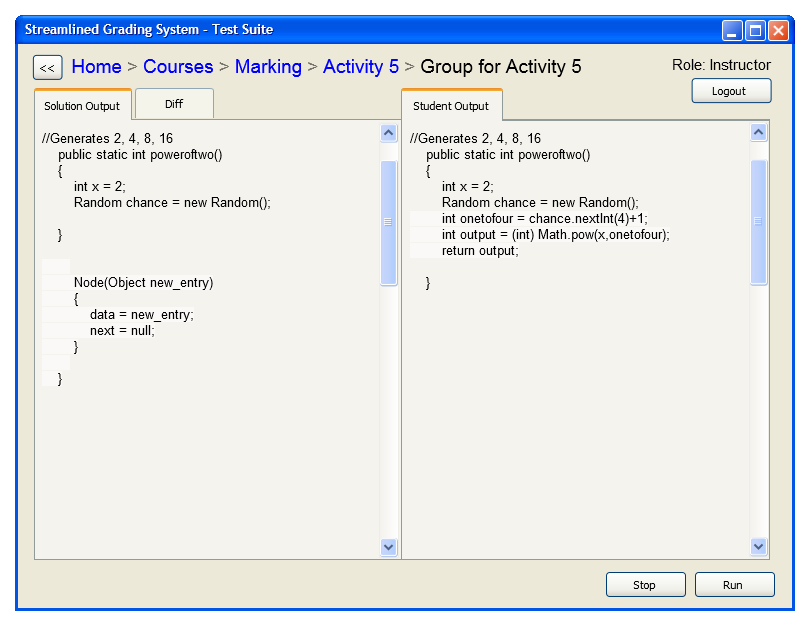
\includegraphics[scale=0.6]{../images/UIMockups/PNG_Renders/SRS_TestSuite_Split}
\end{center}
The Test Suite shows the \textbf{Solution Output}, the \textbf{Student Output}, and the \textbf{Diff}.  
The three windows can be docked together(tabbed) or positioned that each
window takes up 1/3 of the screen space.
The \textbf{Diff} window intelligently shows the difference between
solution and submitted code.

\subsection{Manage Database}

\subsection{Manage User Accounts}

\subsection{Manage System Logs}

% ---
\section{Quick Reference}  % 9 Marks

% ---
\section{Known Bugs}
There are no bugs, our software is perfect.

\end{document}
